%!TEX root = paper.tex



In the previous section, we demonstrated that DeepER provides superior prediction performance than the baseline models. In this section, we discuss some additional learnings from our exploration of this dataset.

\subsection{Qualitative Results}

 We next discuss the qualitative prediction performance of DeepER  as well as the baselines.  Figure \ref{fig:qualitative} shows  the 1-step prediction performance for DeepER, ARIMA, and linear regression for \textit{Fire}.  From the figure, we observe that all models  struggle to predict the values accurately.  From our experience of working with similar models in the past  \cite{SWaP, DeepFit, 8884240}, we have observed that sequence-to-sequence models are generally able to make really superior predictions. This does not appear to be the case always for this prediction task primarily because of the challenging non-periodic and non-seasonal nature  of the emergency events dataset. 
 
 We  observe from Figure \ref{fig:qualitative} that the resolution times for some events is significantly higher in comparison to majority of the points. Because of this pattern, any prediction model  will find it difficult to accurately predict such high peaks. But, despite this  challenging nature of the dataset,  we observe that DeepER   provides a significantly smoothened prediction performance in comparison to the baselines and accurately predicts the underlying pattern. If we overlook the peaks, we can see that  the prediction performance of DeepER for the remaining data points is good. 
 
 In comparison, we observe that the next step predictions for both ARIMA and Linear Regression closely mirror the  actual resolution time  of the previous time step. This occurs because both these baselines only use the past trend to predict the future. This is the root cause behind their poor performance because the  resolution time of the current request is significantly different from the previous one.
 
% As discussed before, due to the events not occurring in fixed time intervals, it is difficult to learn the exact pattern for this dataset.% and hence the predictions do not perfectly match the actual response times, but they try hard to learn the variational patterns from the data. %As mentioned in Section \ref{sec:data}, each incident type has between 29 and 73 sub types. These sub types have response times in different ranges. This leads to high variation in data. Also, as emergency events do not occur in a fixed pattern, the response times are recorded as the incidents are encountered and they are not in fixed time intervals. 

%Besides, the variation in the data due to peaks representing large response times and occurrence of incidents in dynamic length intervals makes forecasting a challenging task. Though DeepER does not accurately predict all the actual response times as seen in Figure \ref{fig:qualitative}, it does predict in a more consistent manner trying to learn the pattern given the complexity of the dataset.



%\begin{figure}[!ht]
%  \centering
%  \subfloat[Fire]{%
%  	\label{fig:qualfire}
%       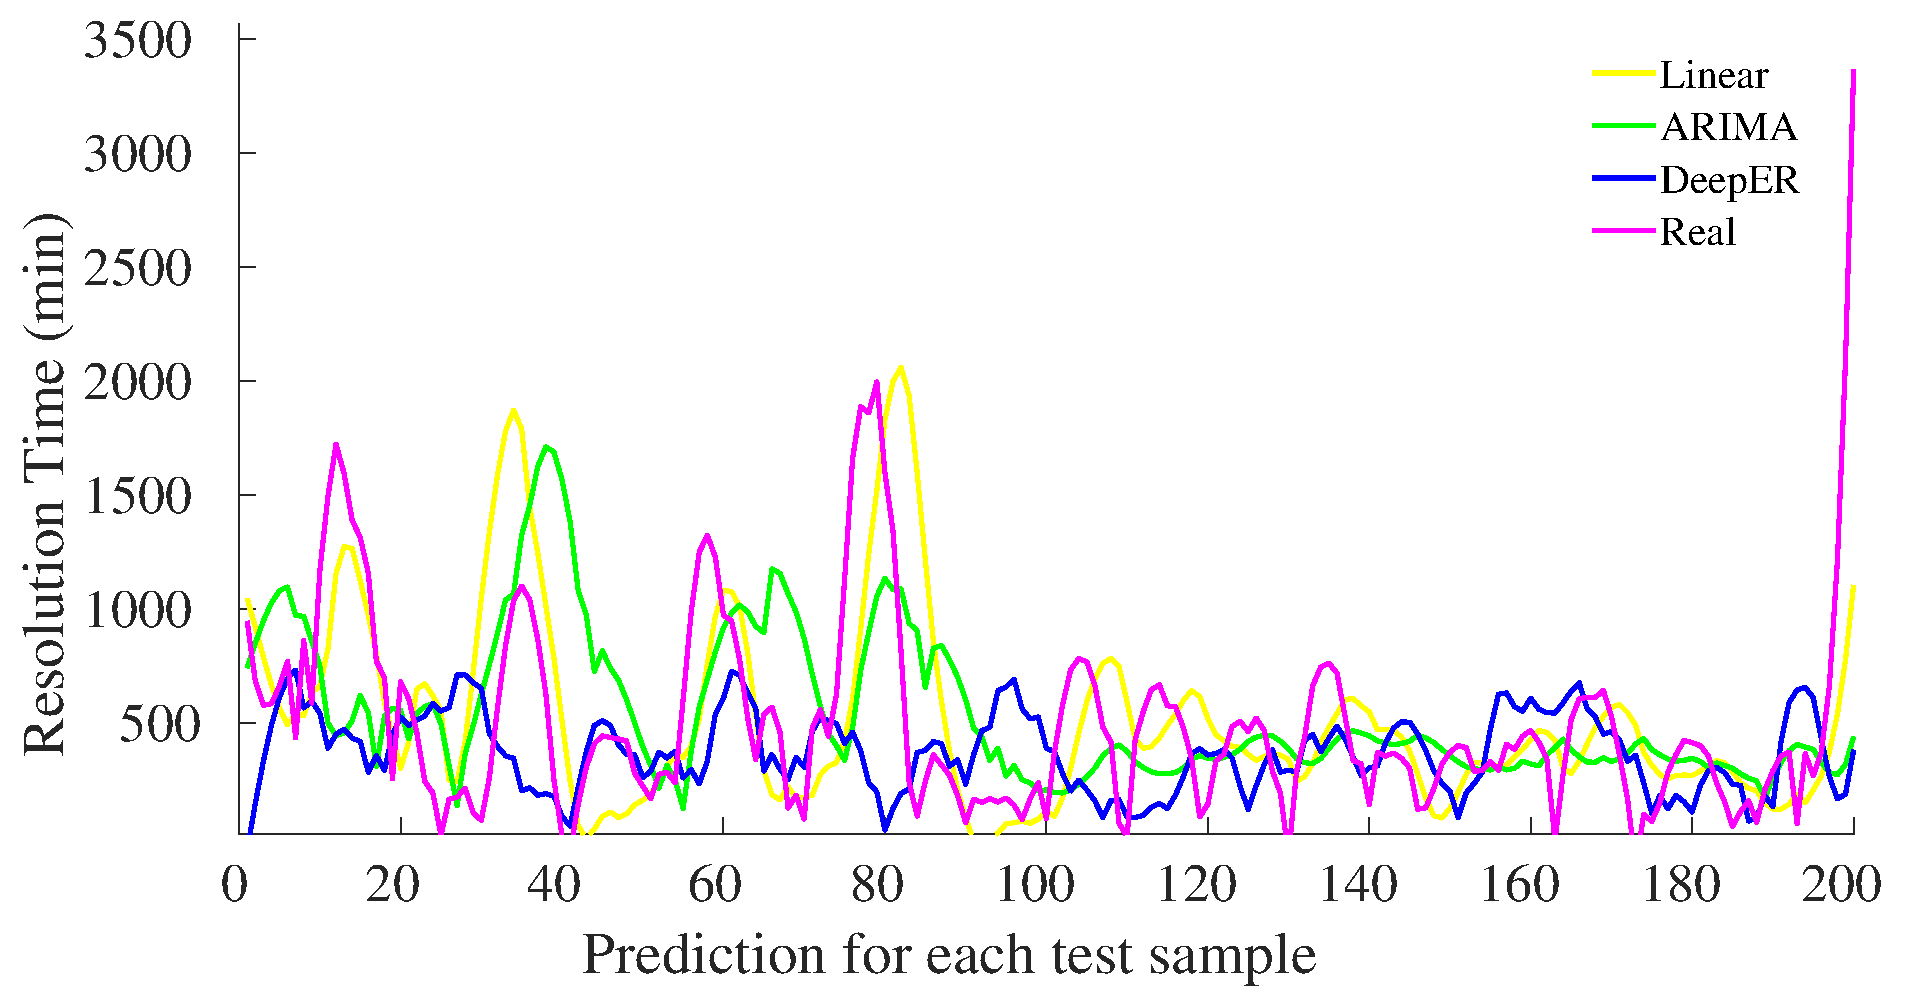
\includegraphics[width=0.9\columnwidth]{Figures/15_5/Dist/1Fire_main_5}
%       }
%  \hfill
%    \subfloat[Law]{%
%         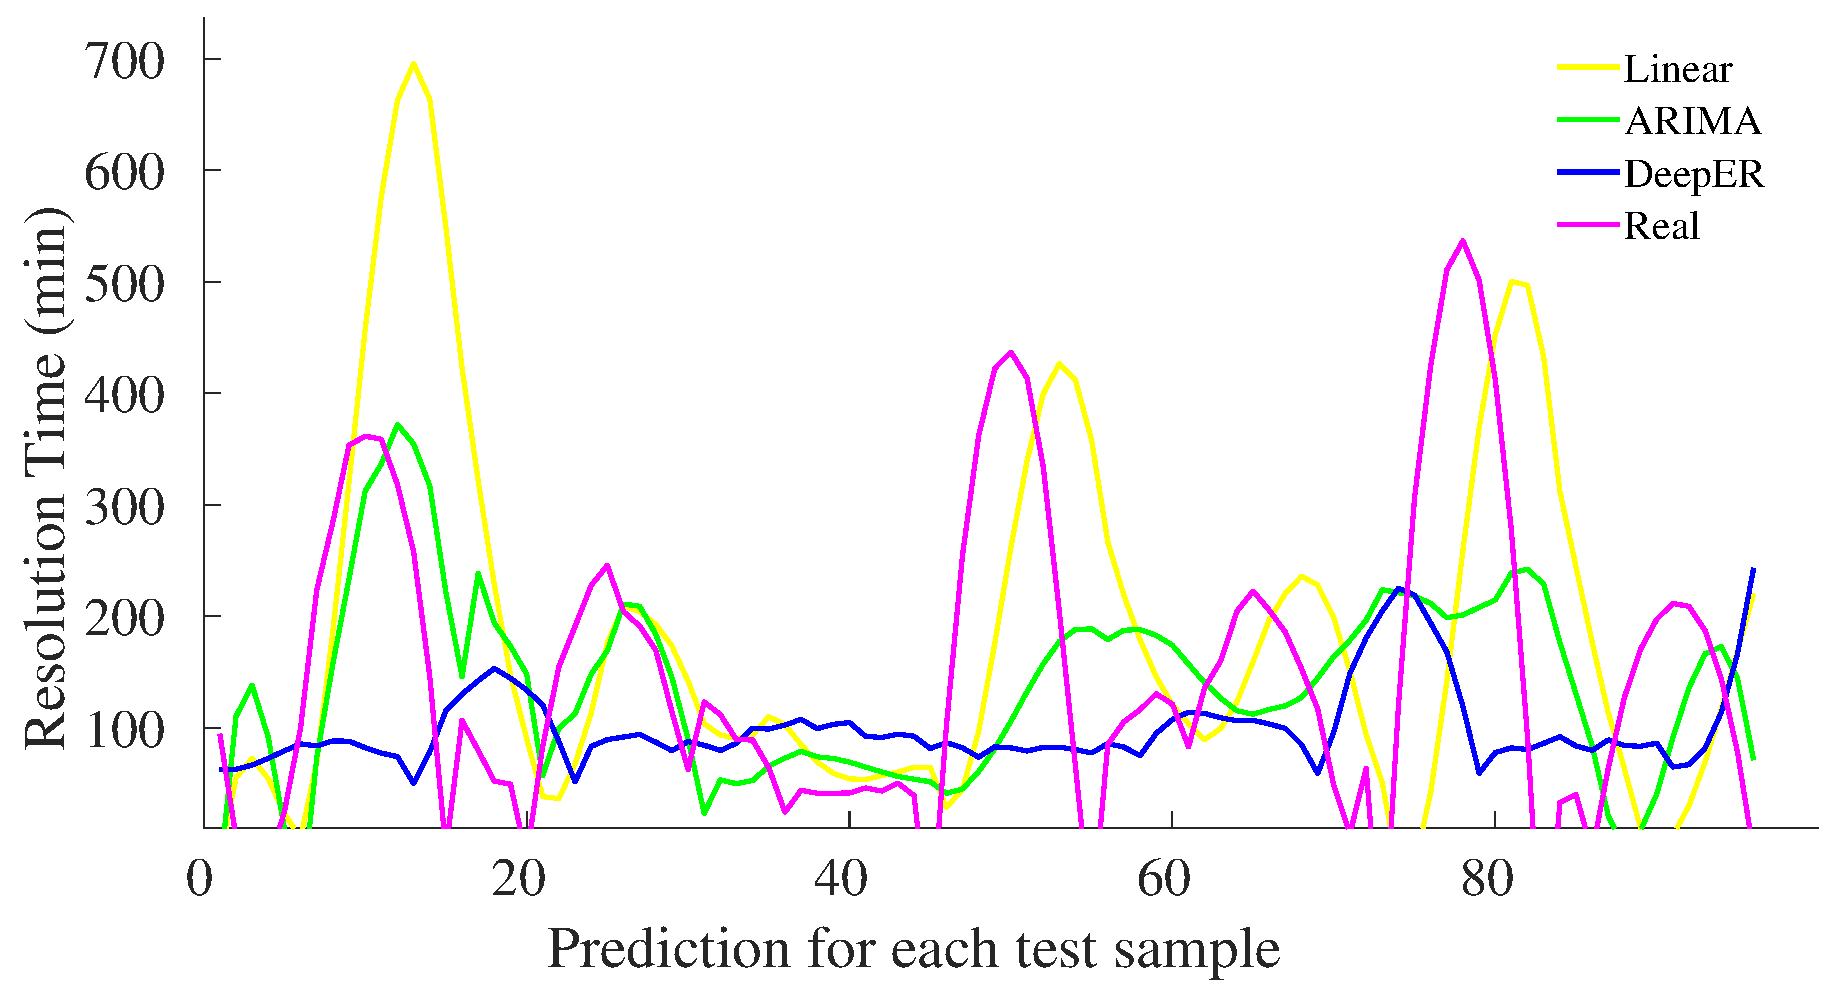
\includegraphics[width=0.9\columnwidth]{Figures/15_5/Dist/1Law_main_6}
%         \label{5b}}
%    \hfill
%  \subfloat[Structural]{%
%       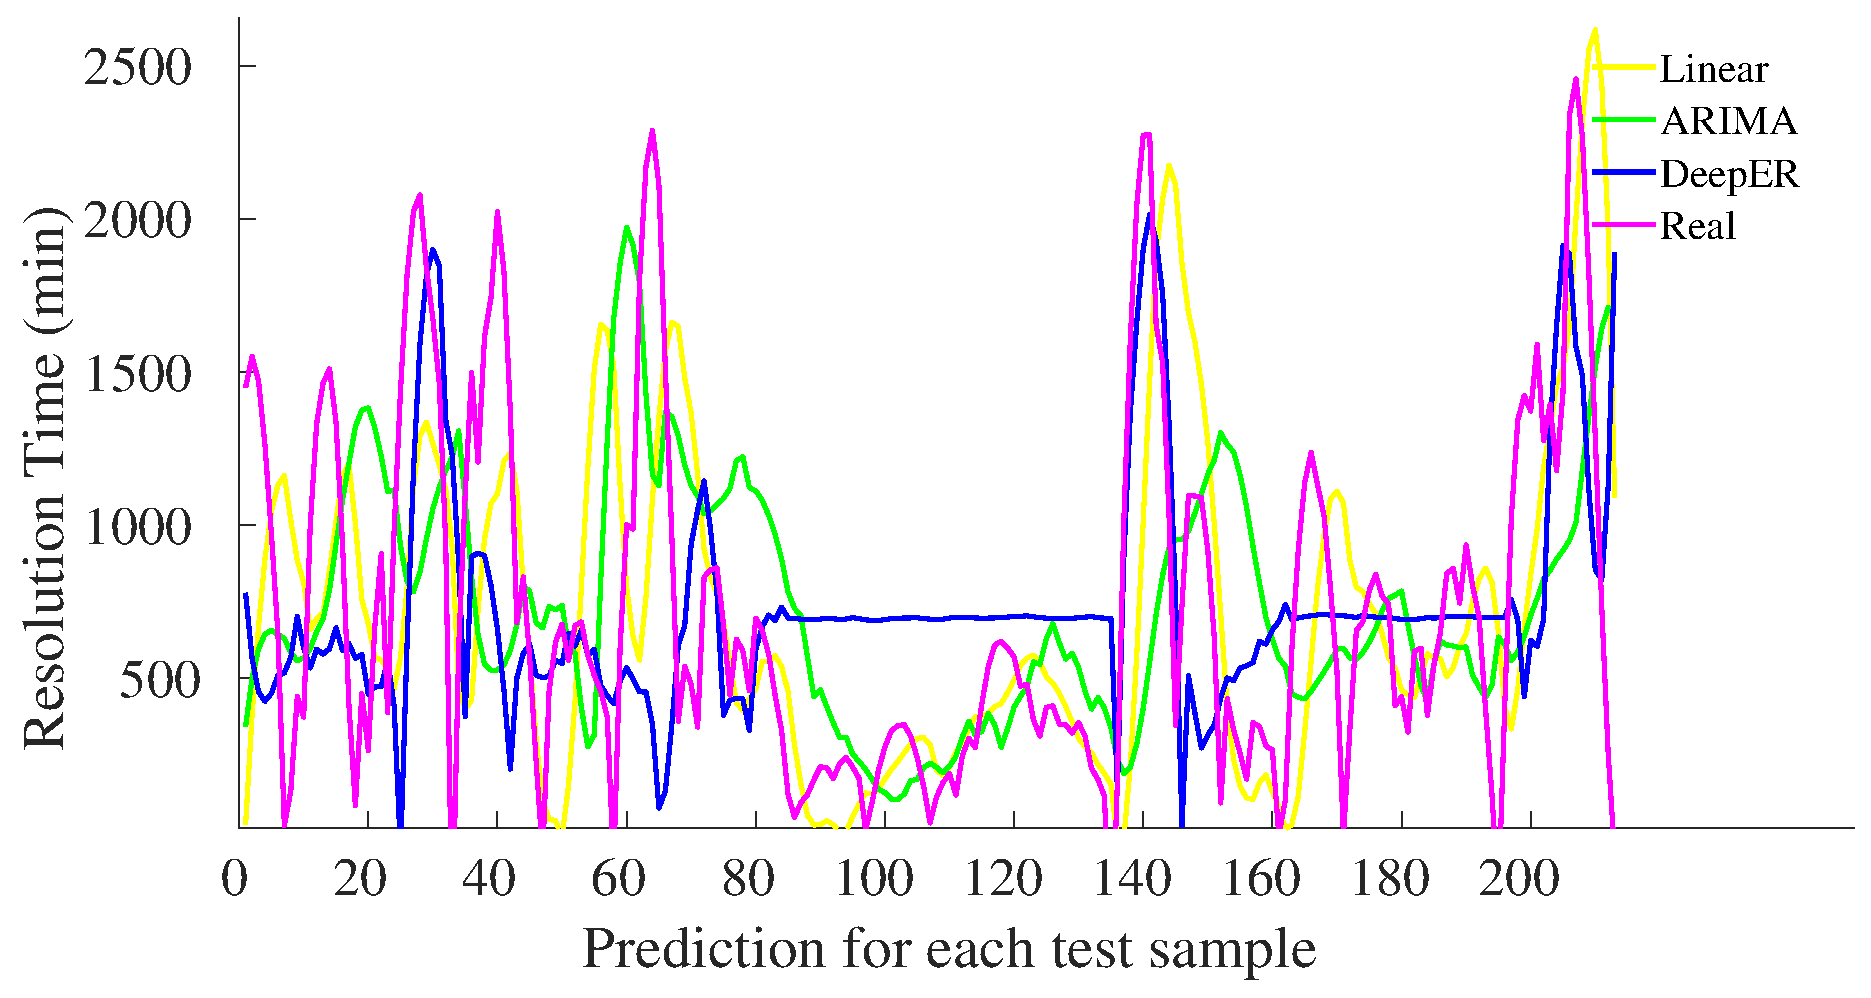
\includegraphics[width=0.9\columnwidth]{Figures/15_5/Dist/1Structural_main_7}
%       \label{5b}}
%	\caption{Real vs Predicted Fire, Law and Structural Comparison of baselines and our approach}
%  \label{fig:qualitative} 
%  \vspace{-3mm}
%\end{figure}

\begin{figure}[!ht]
  \centering
  	\label{fig:qualfire}
       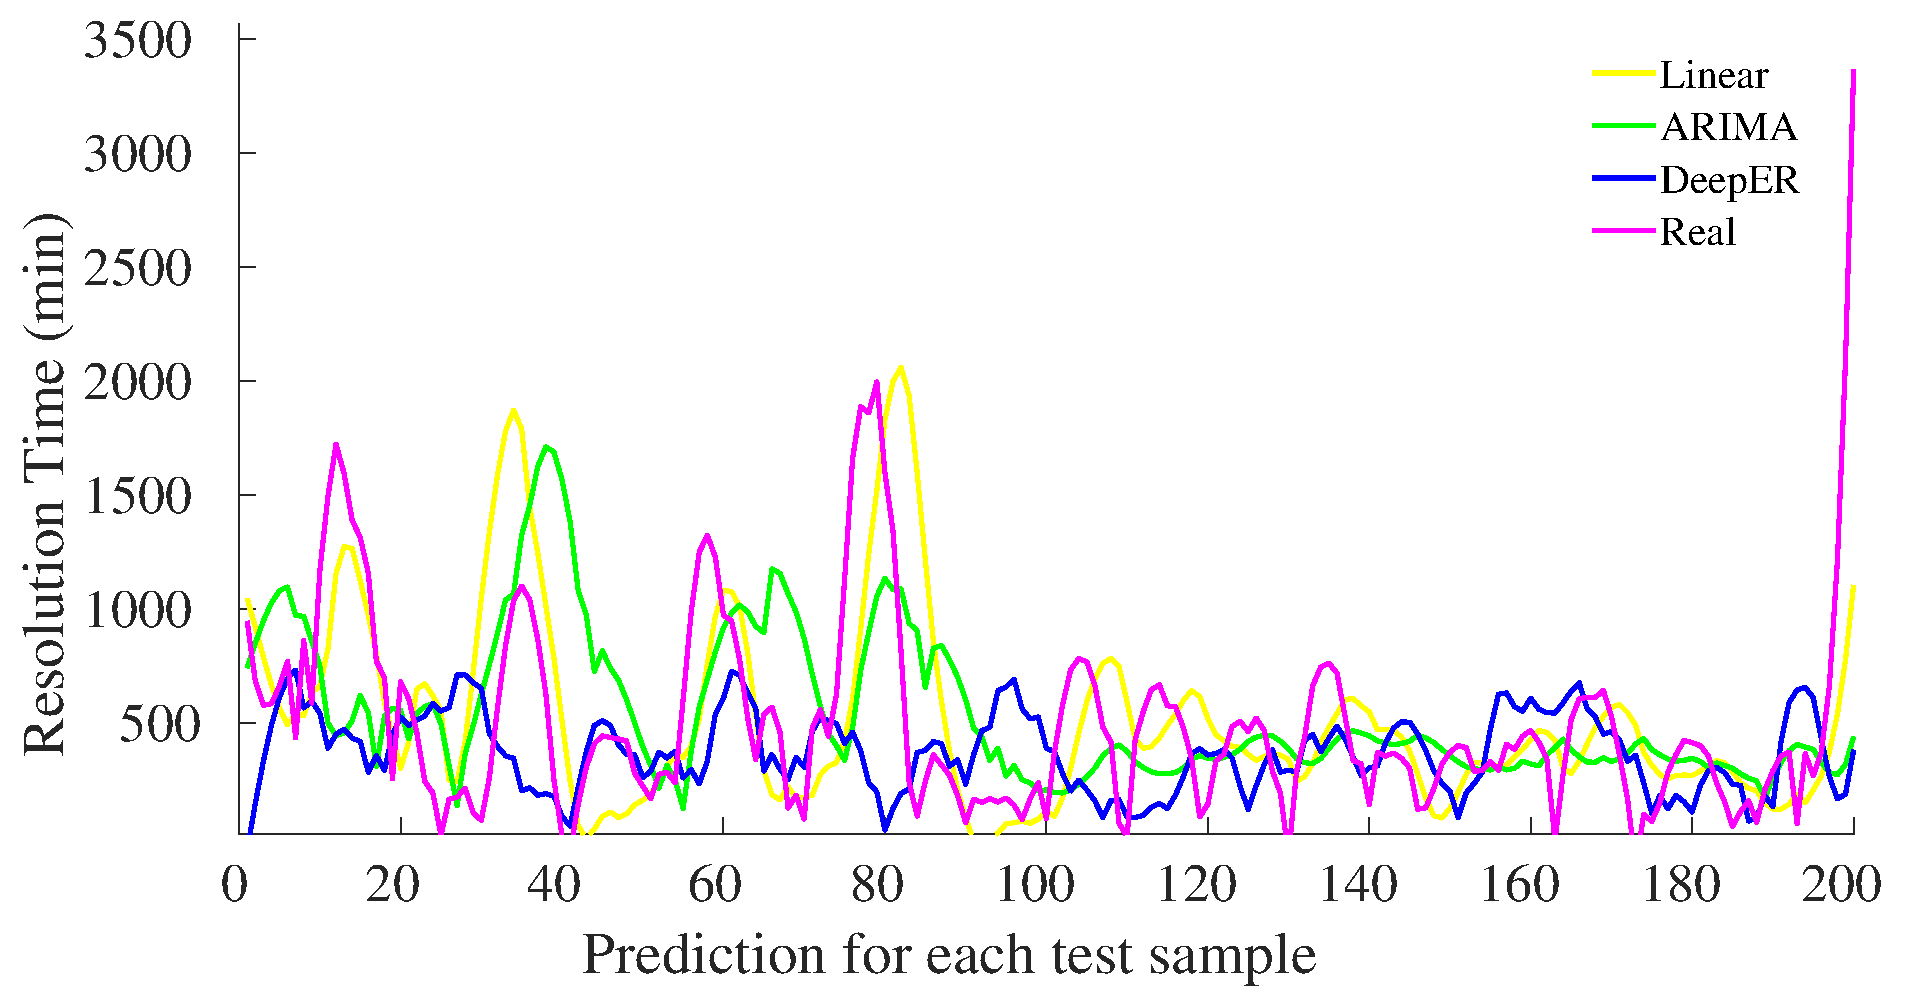
\includegraphics[scale=0.25]{Figures/15_5/Dist/1Fire_main_5}
	\caption{Fire: One step Real vs Predicted Performance}
  \label{fig:qualitative} 
  \vspace{-3mm}
\end{figure}





\subsection{Further Insights into Data Preprocessing}

As mentioned in Section \ref{Data:Preprocessing}, we ensure that the training, validation, and test data include sequences from all years of the dataset. While cross-validation is commonly used to establish the significance of the results, we design this well-crafted split of the dataset to render greater credibility to our results primarily because of the fairly limited number of data points. Additionally, as noted earlier, the dataset contains a non-trivial number of outliers and missing values.  Table \ref{table:outmiss2} shows the number and  percentage of missing and outlier points in each of the training, validation and test sets if the data is split chronologically. This uneven distribution of the outlier and missing values further necessitates a carefully constructed split to ensure that training, validation, and test sets contain a more uniform distribution of such points. We note that while the dataset is relatively small in size, each event corresponds to an emergency and therefore, it is crucial to use all available data points and generate superior predictions because such predictions are critical to improving human safety. 



\begin{table}[!ht]
\centering
\resizebox{\columnwidth}{!}{
\vspace{3mm}
\begin{tabular}{|c|c|c|c|c|}
\hline
\multicolumn{2}{|c|}{\textbf{Incident Type}}&\textbf{Training}&\textbf{Validation}&\textbf{Testing}\\
\hline
%\textbf{Incident Type}& &\textbf{Num Points}& \textbf{\% Out}& \textbf{\% Missing}\\
%\hline
\multirow{3}{*}{Fire} & Total& 1529  & 764  &764\\
&Outliers &8\% &6\%&5\%\\
&Missing &14\% &47\%&53\%\\
\hline
\multirow{3}{*}{Law} & Total& 519  & 260  &260\\
&Outliers &8\% &6\%&13\%\\
&Missing &2\% &17\%&27\%\\
\hline
\multirow{3}{*}{Structural} & Total& 754  & 377  &377\\
&Outliers &8\% &6\%&13\%\\
&Missing &2\% &17\%&27\%\\
\hline
%\multirow{3}{*}{Utility}  & Total& 942  & 471  &471\\
%&Outliers &9\% & 7\% & 6\%\\
%&Missing &2\% & 33\% & 56\%\\
%\hline
\end{tabular}
}
\caption{Statistics of Outliers and Missing values in a Chronological Split}
\label{table:outmiss2}
\vspace{-5mm}
\end{table}




\subsection{Limitations of Enriching DeepER}

We observe from Section \ref{sec:data} that each incident type consists of multiple subtypes. We attempt to perform resolution time prediction at the subtype level, but realize that because this is an emergency  events dataset, the number of data points  is not sufficient for training, validation, and testing of deep learning models for  each subtype separately. We also use these subtypes as features in DeepER, but observe that this enhanced model did not improve prediction performance. We believe that dearth of data at the subtype level is the primary reason behind it not contributing to DeepER's prediction performance.

\subsection{Practicality of DeepER}

With the increase in computational power over the last decade, deploying deep learning based systems to solve real-world problems is becoming relatively easy. As is the case with most deep learning models, DeepER requires some computational time for training. However, once trained, DeepER requires limited amount of  time to generate predictions, a desired attribute in a practical system. Additionally, as more data becomes available, DeepER can be easily retrained thus enabling it to adapt to changing situations. We anticipate DeepER to be retrained at comparatively infrequent intervals (i.e., only when significant number of new emergency events have been resolved).



%The usual split in chronological order, train, validation, test, made the percentage of invalid points (outliers and missing values) in the validation and test set at least triplicate the percentage of missing values in the training set for all the group types.  This approach lead us to poor quantitative and qualitative results. For this reason, we distritube the replacement of these invalid values fairly among training, validation and test set, as explained in section \ref{sec:data}. Other preprocessing approaches lead us to relative similar quantitative results. One of these approaches was to remove missing values. A second approach was replacing values larger than initial quantile 90 with the quantile 90 value for each incident type.
%%In this section, we add more insights to the visual analysis and support the decisions of spliting in a different way. 
%As a summary, we can say that these approaches generated flat predictions or very similar along the multi-step predicion and among instances. 
%A last approach we tried was to simplify the replacement generation with sampling randonmly from the valid points in each type. We notice that predictions still show the variations that we expected, however RMSE values increased slightly.





